
\section{Ajuste de la torsión geométrica} \label{sec:ajuste_torsion}

En esta sección se ajusta la torsión geométrica del ala para lograr un momento nulo alrededor del centro de gravedad de la aeronave en la condición de diseño, \ie, $C_{M,\text{cg}} = 0$.

La condición de diseño es vuelo horizontal rectilíneo uniforme, \ie, la suma de fuerzas verticales es nula. Con una carga alar $\mathcal{W}/S = 20 \ \kilo\gram / \meter^2$, la masa de la aeronave será $S \cdot \mathcal{W} / S$. El $C_L$ de diseño será
\begin{equation}
    C_{L,\text{d}} = \frac{W}{\rho V^2 S / 2} = 
    \frac{g_0 S \cdot \mathcal{W} / S}{\rho V^2 S / 2} = 
    \frac{g_0 \cdot \mathcal{W} / S}{\rho V^2 / 2}
\end{equation}
En atmósfera ISA a nivel del mar con velocidad de vuelo de $100 \ \kilo\meter / \hour$, $C_{L,\text{d}} = 0.4150$. 

La torsión geométrica $\left( \varepsilon(y) \right)$ se define como el ángulo que forma la cuerda de una sección de ala respecto de la cuerda de la sección raíz. La torsión permite trabajar la distribución de sustentación a lo largo de la envergadura modificando el ángulo de ataque que ve cada sección. De este modo, para un mismo ángulo de ataque, alas con distinta torsión generan sustentaciones distintas. Ello permite modificar la posición del centro de presiones $\left( x_{cp} \right)$ y así el momento sobre el centro de gravedad generado por la sustentación. En este caso se estudiará una ley de torsión lineal, en la que basta con definir la torsión de la sección de punta $\left( \varepsilon_t \right)$. 

Primeramente debe obtenerse la posición del centro de presiones, \ie, el punto de aplicación de la sustentación. Conocidos $C_{L,\text{d}}$ y el momento respecto de LE de diseño, $C_{M_{LE}, \text{d}}$,
\begin{equation} \label{eq:calculo_xcp}
    \frac{x_\text{cp}}{\overline{\overline{c}}} = 
    - \frac{C_{M_{LE}, \text{d}}}{C_{L,\text{d}}}
\end{equation}
El momento respecto del centro de gravedad es la contribución del momento libre del ala $\left( C_{M0} \right)$ y el generado por la sustentación,
\begin{equation} \label{eq:calculo_cmcg}
    C_{M_\text{cg}} = 
    C_{M0} - C_L \frac{x_\text{ac} - x_\text{cg}}{\overline{\overline{c}}}
\end{equation}
donde el centro aerodinámico $\left( x_\text{ac} \right)$ y el momento libre se obtienen mediante
\begin{gather}
    \frac{x_\text{ac}}{\overline{\overline{c}}} = 
    - \frac{d C_{M_\text{LE}}}{d C_L} \\
    C_{M0} = C_L \frac{x_\text{ac} - x_\text{cp}}{\overline{\overline{c}}} \label{eq:calculo_CM0}
\end{gather}

Numéricamente se obtienen los coeficientes de fuerzas y momentos del ala para torsiones entre $-12\degrees$ y $0\degrees$, y ángulos de ataque entre $-2\degrees$ y $10\degrees$, para $N = 200$. Se calcula la regresión de $C_{M_\text{LE}} = f \left( C_L \right)$ y se obtienen $x_\text{ac}$ y el coeficiente de momento respecto de LE en condición de diseño $\left( C_{M_\text{cg},\text{d}} \right)$. Con \eqref{eq:calculo_xcp} se calcula $x_\text{cp}$, con \eqref{eq:calculo_CM0} se calcula el momento libre y con \eqref{eq:calculo_cmcg} el coeficiente de momento en condición de diseño. También se calcula el ángulo de ataque en condición de diseño $\left( \alpha_\text{d} \right)$. Cuando $C_{M_\text{cg},\text{d}}[i] \cdot C_{M_\text{cg},\text{d}} [i+1] < 0$, existe un $\varepsilon_t$ entre $\varepsilon[i]$ y $\varepsilon[i+1]$ tal que $C_{M_\text{cg},\text{d}} = 0$. Dada la linealidad del problema, $C_{M_\text{cg},\text{d}} = f \left( \varepsilon_t \right)$ y $\alpha_\text{d} = f \left( \varepsilon_t \right)$ son lineales. Interpolando entre $\varepsilon[i]$ y $\varepsilon[i+1]$ se obtiene la torsión adecuada. 

La solución obtenida con el método propuesto es $\varepsilon_t = -4.3677 \degrees \approx -4.40 \degrees$ y $\alpha_d = 5.6706 \degrees \approx 5.70 \degrees$.

En la figura \ref{fig:trim_wing} se representa el coeficiente de momento respecto de CG y el ángulo de ataque en condición de diseño en función de la torsión en la punta de ala.

\begin{figure}[h]
    \centering
    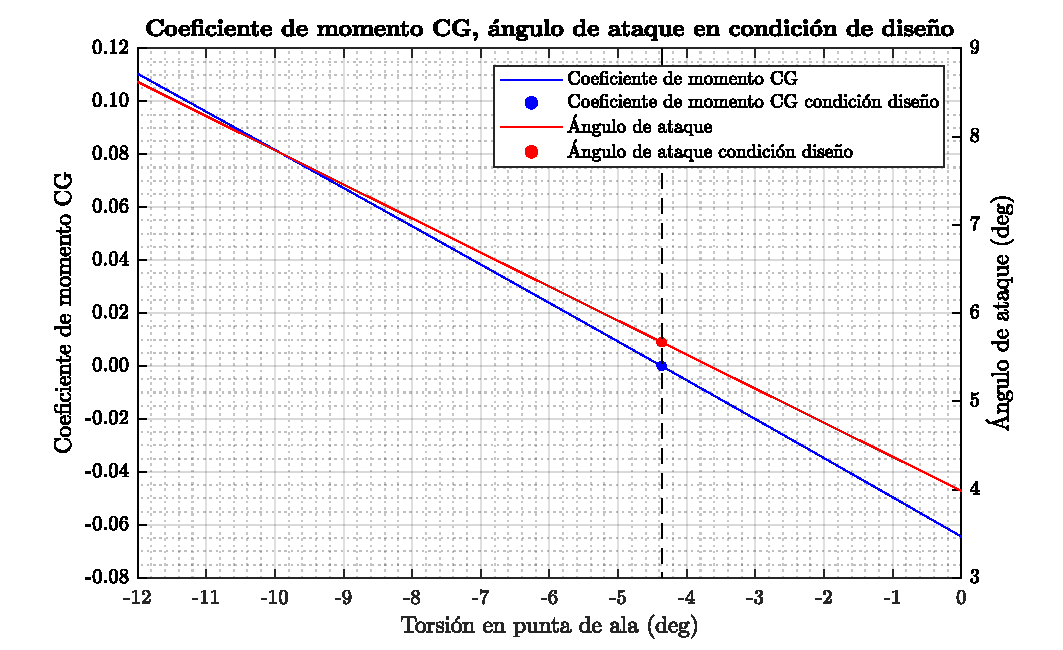
\includegraphics[width=\linewidth]{imagenes/ajuste_torsion/trim_wing.pdf}
    \caption{Coeficiente de momento respecto CG $( C_{M_\text{cg}} )$ y ángulo de ataque de diseño $\left( \alpha_\text{d} \right)$ en condición de diseño, en función de la torsión geométrica en punta de ala $\left( \varepsilon_t \right)$.}
    \label{fig:trim_wing}
    \vspace{-4mm}
\end{figure}

En la sección \ref{sec:distribucion_lift} se explica la función de la torsión geométrica del ala para lograr $C_{M_\text{cg}} = 0$, en base a las distribuciones de sustentación básica y adicional.












